\documentclass{beamer}

\usepackage{beamerthemesplit}
\usepackage{latexsym}
\usepackage{eurosym}
\usepackage[activeacute,spanish]{babel}
\usepackage{ae,aecompl}
\usepackage{graphicx}
\usepackage{amsfonts}

\usetheme{Darmstadt}

\title{EMACS IDE}
\author{Alejandro Cardona \\ Felipe Gongora}
\date{\today}

\begin{document}

\frame{\titlepage}

\section[\'Indice]{}
\begin{frame}[allowframebreaks]
\tableofcontents
\end{frame}
%\frame{\tableofcontents}

\section{EMACS}
\begin{frame}[allowframebreaks]
\frametitle{Introducci\'on}
Emacs es un editor de texto con una gran cantidad de funciones, muy popular entre programadores y usuarios t\'ecnicos. Gnu Emacs es obviamente parte del proyecto GNU y la versión m\'as popular de Emacs con una gran actividad en su desarrollo. El manual de GNU Emacs lo describe como un editor \textbf{extensible, personalizable, auto-documentado y de tiempo real}.
\begin{center}

\includegraphics[height=0.3\textheight]{img/emacs.png}
\end{center}
\end{frame}

\begin{frame}[allowframebreaks]
\frametitle{Lenguajes en Emacs}
\begin{itemize}
\item
c 
\item
c++ 
\item
c# 
\item
perl 
\item
python 
\item
ruby 
\item
SQL 
\item
LaTeX 
\item
HTML 
\item
CSS 
\item
etc
\end{itemize}
\end{frame}

\begin{frame}[allowframebreaks]
\frametitle{Interfaz grafica}
\begin{center}
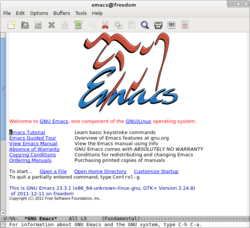
\includegraphics[height=0.8\textheight]{img/interfaz.png}
\end{center}
\end{frame}

\section{Emacs como ide}
\begin{frame}[allowframebreaks]
\frametitle{IDE}
Debido a la gran capacidad de configuraci\'on y personalizaci\'on de EMACS, este editor nos permite instalar paquetes adicionales que proporcionan herramientas, para tener una configuraci\'on de IDE para el lenguaje que se desee, a dem\'as de proporcionarnos herramientas de depuraci\'on, identacion, compilaci\'on en tiempo real etc.
%\begin{center}
\begin{figure}[h]
\centering
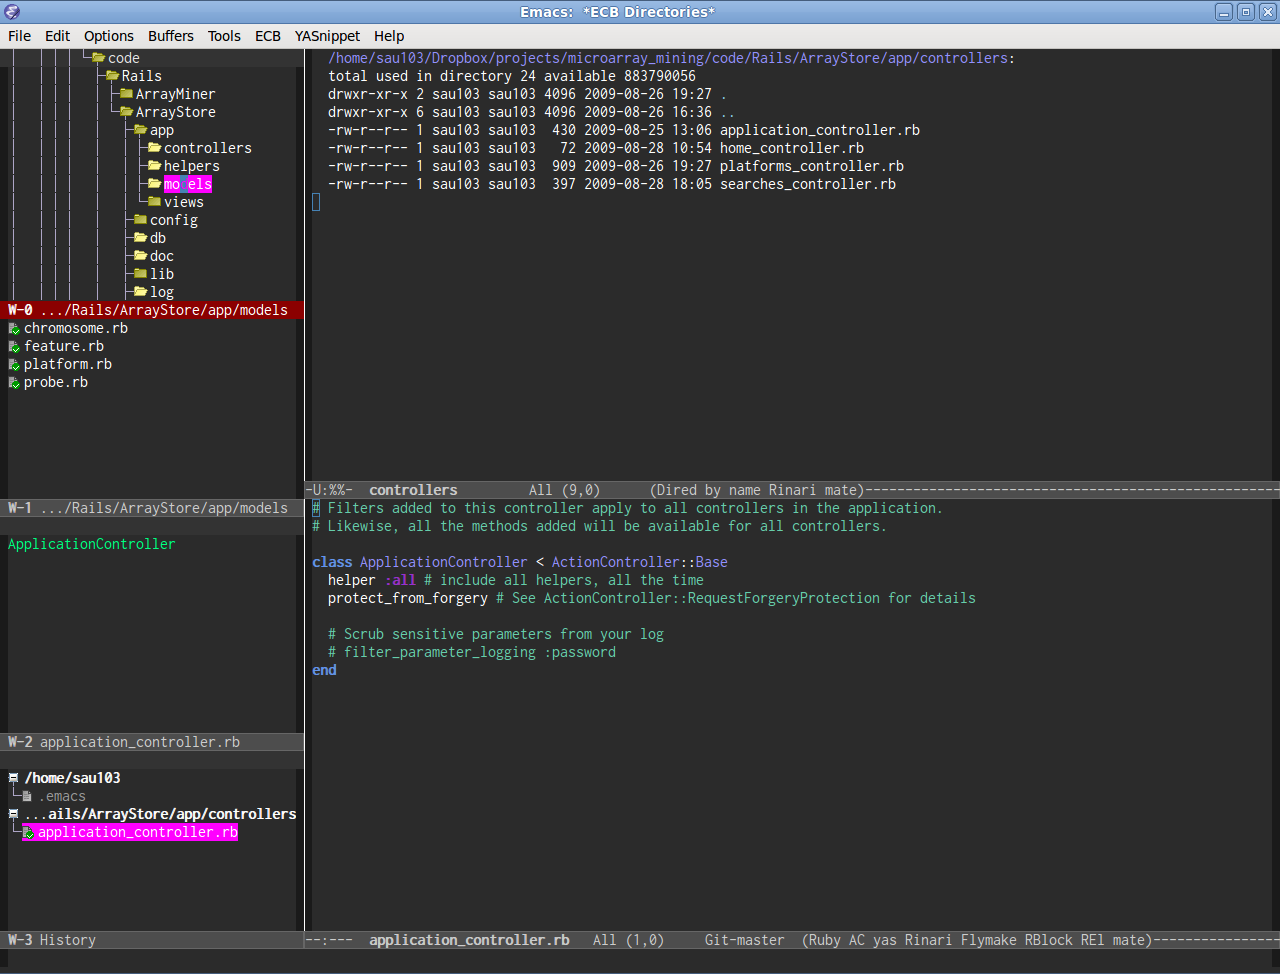
\includegraphics[height=0.3\textheight]{img/conf.png}
\end{figure}
%\end{center}
\end{frame}

\begin{frame}[allowframbreaks]
\frametitle{Sección 2b}
\end{frame}

\begin{frame}[allowframbreaks]
\frametitle{Sección 3b}
\end{frame}

\section{Seccion4}
\frame[allowframebreaks]{
\frametitle{Sección 4}

\begin{enumerate}
\item Punto 1
\item Punto 2
\end{enumerate}

\begin{figure}[h]
\centering
%\includegraphics[height=0.5\textheight]{figure.png}
\caption{Figura}
\label{figure}
\end{figure}

}

\end{document}


